%---------------------------------------------------------------------------%
\lecture{Research Presentation}{lec_present_method}
%---------------------------------------------------------------------------%
\section{Analisi}
%---------------------------------------------------------------------------%
\begin{frame}[fragile]
\frametitle{Prime Analisi: Income}
\begin{table}[H]
\centering
\begin{tabular}{rlrr}
  \hline
 & variable & n\_miss & pct\_miss \\ 
  \hline
1 & Income &  24 & 1.07 \\ 
  2 & ID &   0 & 0.00 \\ 
  3 & Year\_Birth &   0 & 0.00 \\ 
  4 & Education &   0 & 0.00 \\ 
  5 & Marital\_Status &   0 & 0.00 \\ 
  6 & Kidhome &   0 & 0.00 \\ 
  7 & Teenhome &   0 & 0.00 \\ 
  8 & ... & ... & ... \\
   \hline
\end{tabular}

    \caption{Output funzione \textit{miss\_var\_summary(dataSet)}}
   
   \label{fig:miss_var_summary(dataSet)}
\end{table}
\end{frame}
%---------------------------------------------------------------------------%
\begin{frame}[fragile]
\frametitle{Prime Analisi: Z\_CostContact e Z\_Revenue}
\begin{figure}[H]
  \centering
  \begin{minipage}[b]{0.35\textwidth}
    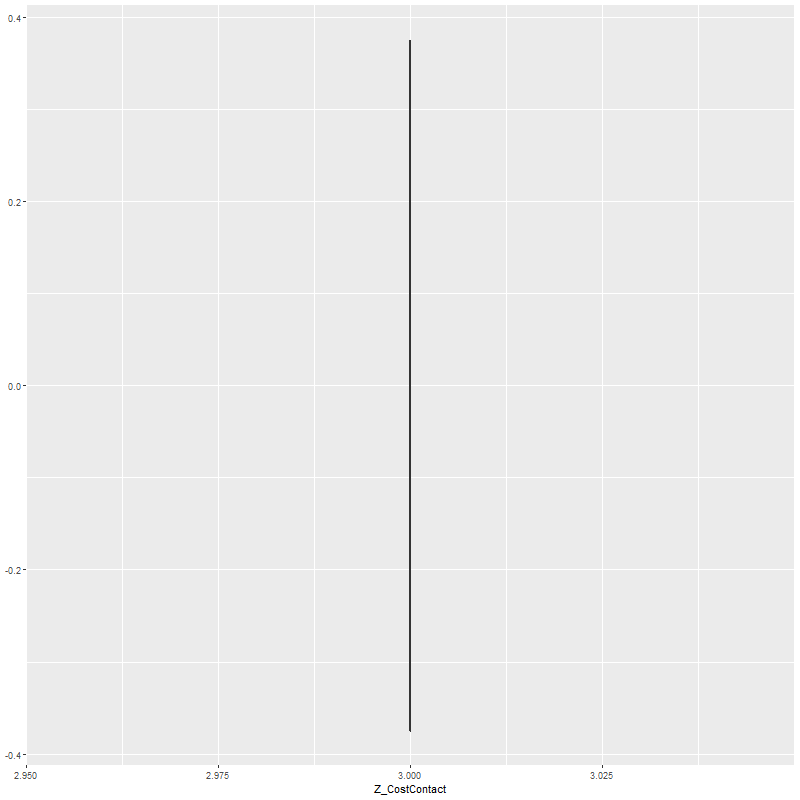
\includegraphics[width=\textwidth]{Img/DESCRIPTION018.png}
    \caption{BoxPlot Z\_CostContact}
    \label{fig:ZRevenue}
  \end{minipage}
  \hspace{5em}
  \begin{minipage}[b]{0.35\textwidth}
    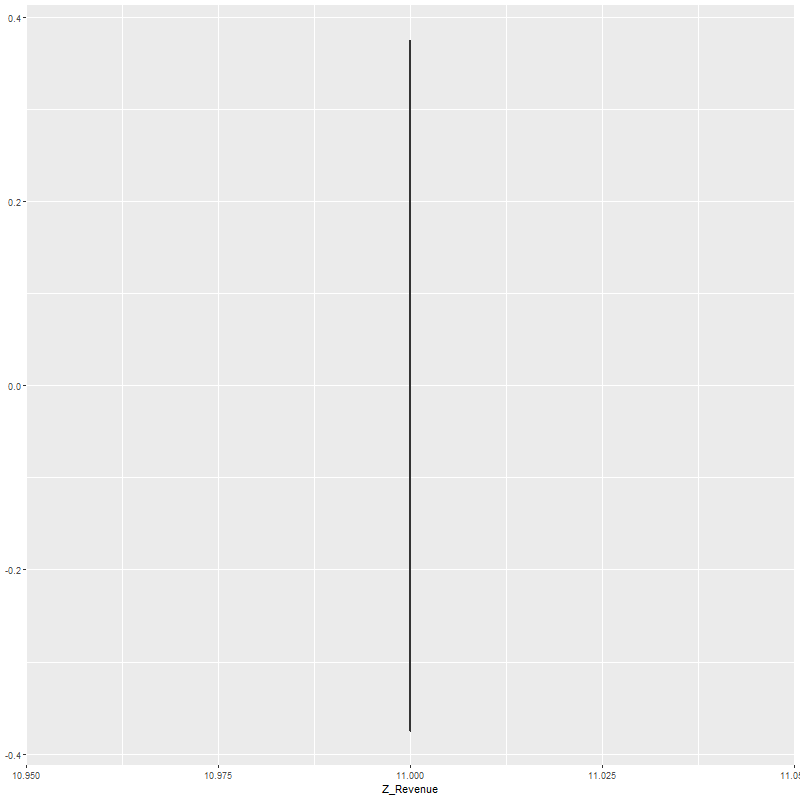
\includegraphics[width=\textwidth]{Img/DESCRIPTION019.png}
    \caption{BoxPlot Z\_Revenue}
      \label{fig:ZCostContact}
  \end{minipage}
\end{figure}
\end{frame}
%---------------------------------------------------------------------------%
\begin{frame}[fragile]
\frametitle{DataPreprocessing}
\begin{enumerate}
    \item Refactor del dataset
    \item Risoluzione dei valori mancanti nella variabile \textit{income}
    \item Splitting del dataset in \textit{trainingSet} e \textit{testSet}
    \item Feature Scaling
\end{enumerate}
\end{frame}
%---------------------------------------------------------------------------%
\begin{frame}[fragile]
\frametitle{Refactor del Dataset}
\begin{enumerate}
    \item Incorporamento dei dati ridondanti
    \item Conversione degli elementi in \textit{factor}
    \item Creazione di nuove variabili riassuntive
        \begin{itemize}
        \item Age
        \item Total\_Spent
        \item Total\_Campains
        \item Total\_Childs
    \end{itemize}
    \item Rimozione delle variabili superflue
    \begin{itemize}
        \item Z\_Revenue
        \item Z\_CostContact
        \item ID
        \item Dt\_customers
    \end{itemize}
\end{enumerate}
\end{frame}
%---------------------------------------------------------------------------%
\begin{frame}[fragile]
\frametitle{EDA}
\begin{figure}[!htb]
\minipage{0.32\textwidth}
  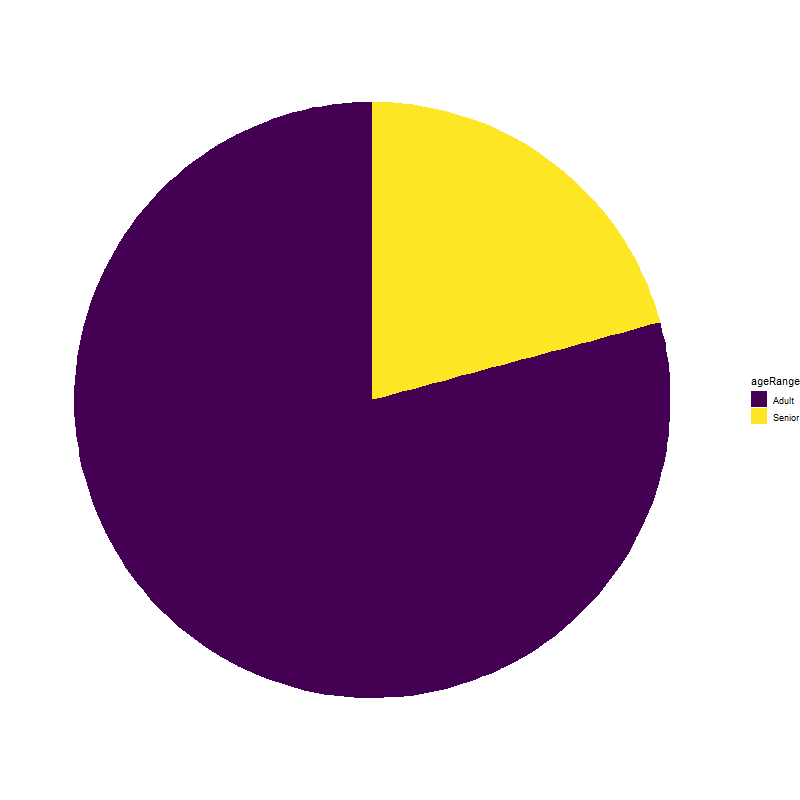
\includegraphics[width=\linewidth]{Img/eda/EDA001.png}
  \caption{Grafico a torta di \textit{Age}}\label{fig:PiePlotAge}
\endminipage\hfill
\minipage{0.32\textwidth}
  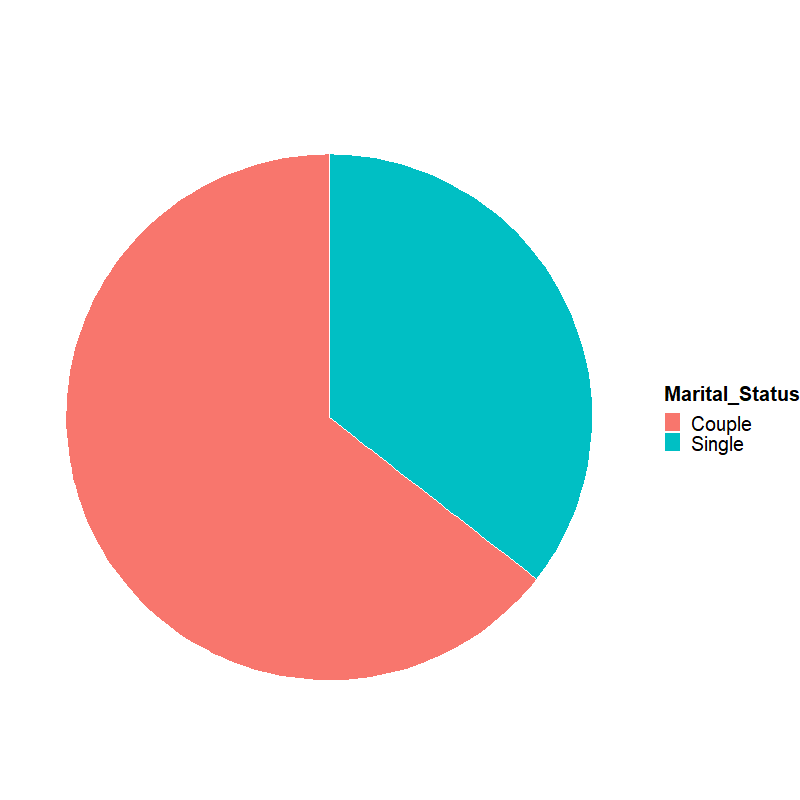
\includegraphics[width=\linewidth]{Img/eda/EDA002.png}
  \caption{Grafico a torta di \textit{Marital\_Status}}\label{fig:PiePlotMt}
\endminipage\hfill
\minipage{0.32\textwidth}%
  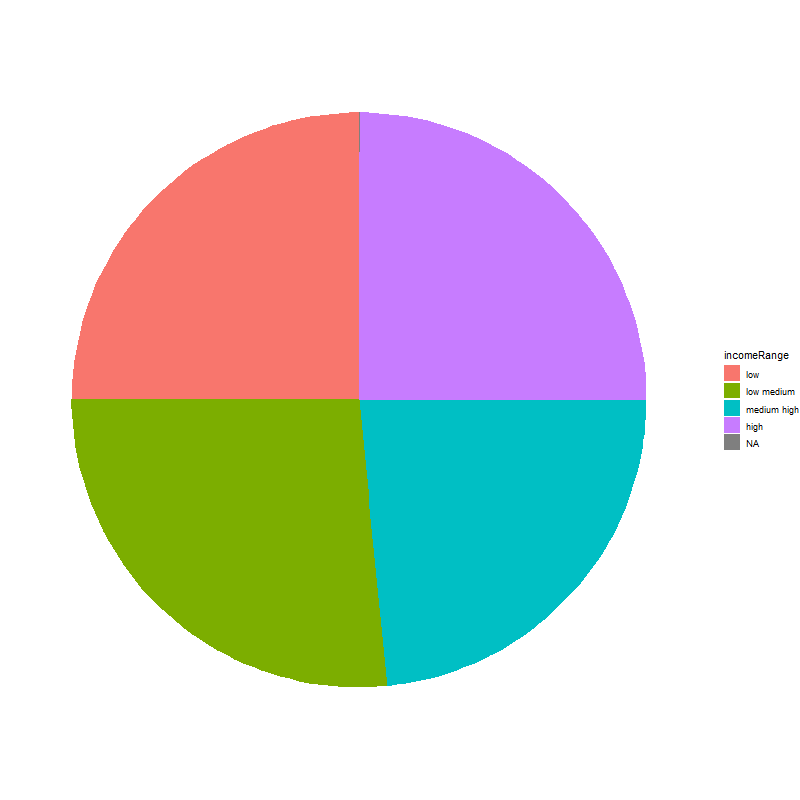
\includegraphics[width=\linewidth]{Img/eda/EDA003.png}
  \caption{Grafico a torta di \textit{Income}}\label{fig:PiePlotIncome}
\endminipage
\end{figure}
\end{frame}
%---------------------------------------------------------------------------%
\begin{frame}[fragile]
\frametitle{EDA: Age, Education  e Marital\_Status}
\begin{figure}[!htb]
\minipage{0.32\textwidth}
  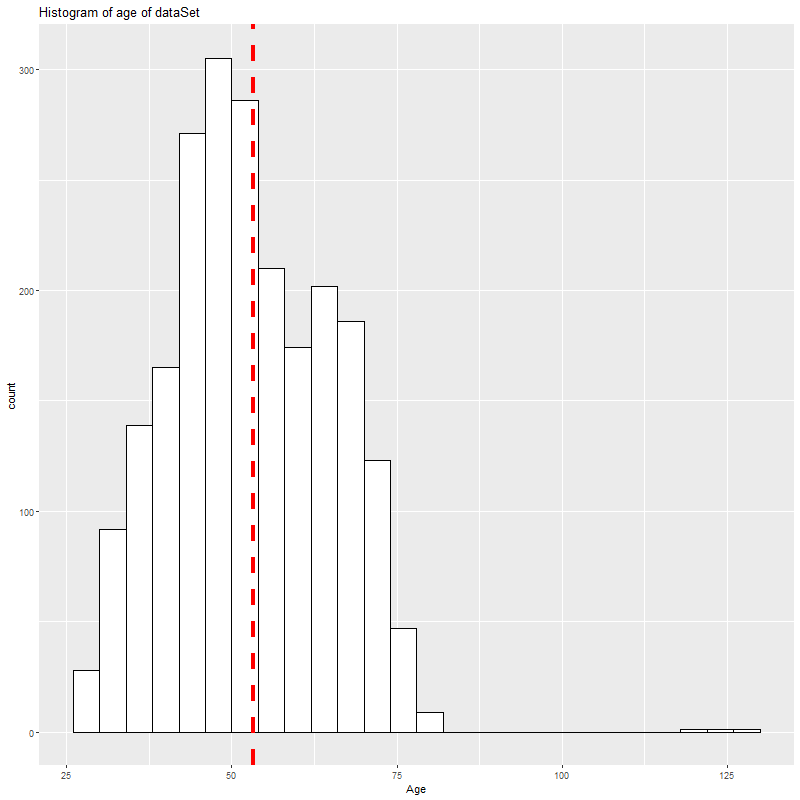
\includegraphics[width=\linewidth]{Img/eda/EDA005.png}
  \caption{Istogramma di \textit{Age}}\label{fig:HistPlotAge}
\endminipage\hfill
\minipage{0.32\textwidth}
  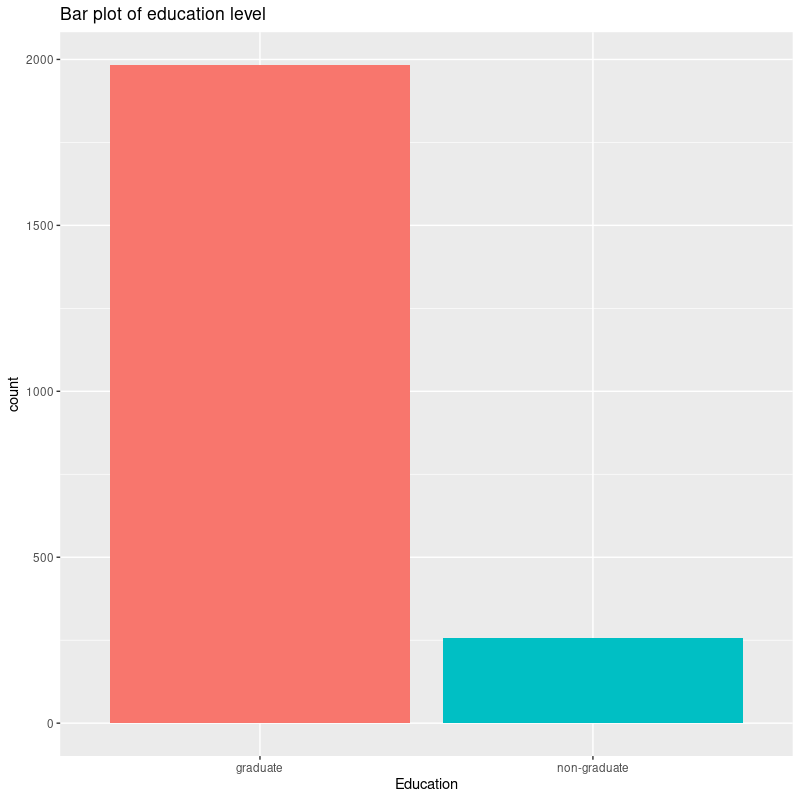
\includegraphics[width=\linewidth]{Img/eda/EDA007.png}
  \caption{Grafico a barre di \textit{Education}}\label{fig:BarPlotEducation}
\endminipage\hfill
\minipage{0.32\textwidth}%
  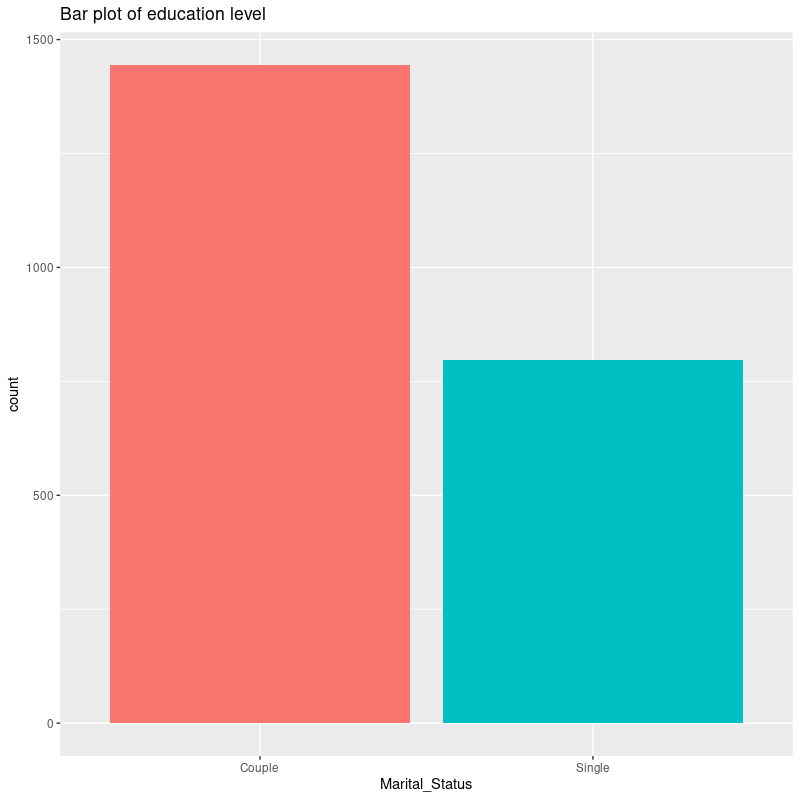
\includegraphics[width=\linewidth]{Img/eda/EDA051.png}
  \caption{Grafico a barre di \textit{Marital\_Status}}\label{fig:BarPlotMt}
\endminipage
\end{figure}
\end{frame}
%---------------------------------------------------------------------------%
\begin{frame}[fragile]
\frametitle{EDA: Istogrammi delle variabili Amount}

    \begin{figure}
    \centering
        \begin{minipage}{.3\textwidth}
            \begin{subfigure}{\textwidth}
            \centering
            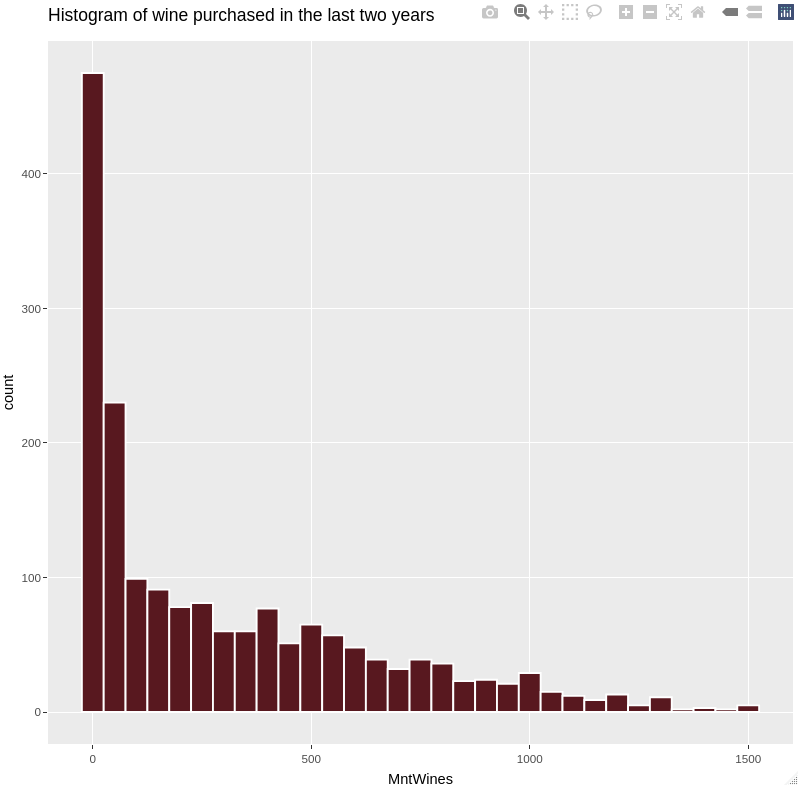
\includegraphics[width=0.7\textwidth]{Img/eda/EDA018.png}
            \end{subfigure}\\
            \begin{subfigure}{\textwidth}
            \centering
            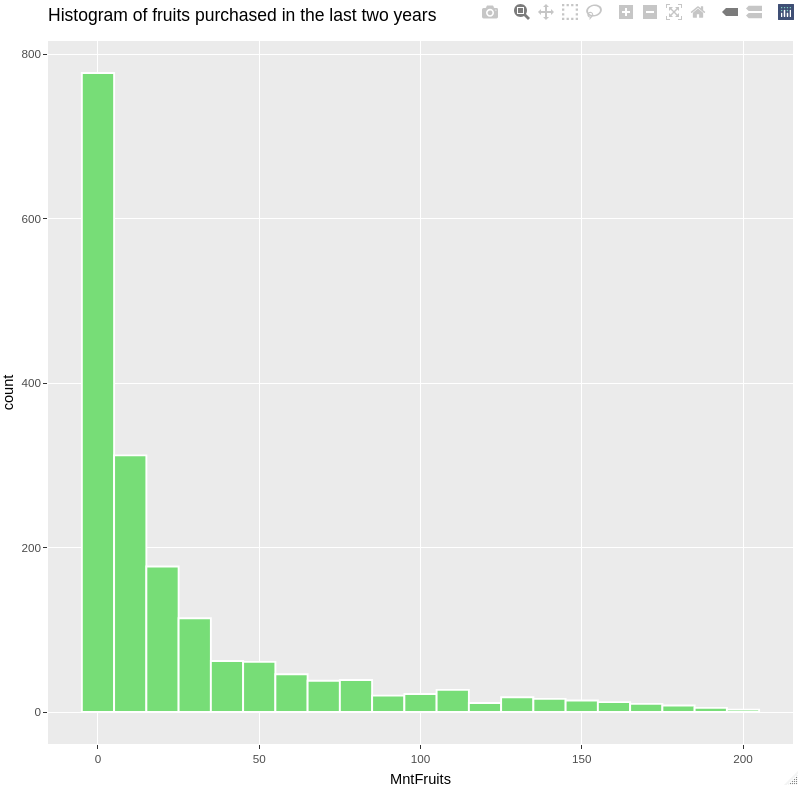
\includegraphics[width=0.7\textwidth]{Img/eda/EDA019.png}
            \end{subfigure}%    
        \end{minipage}
        \hfill
        \begin{minipage}{.3\textwidth}
            \begin{subfigure}{\textwidth}
            \centering
            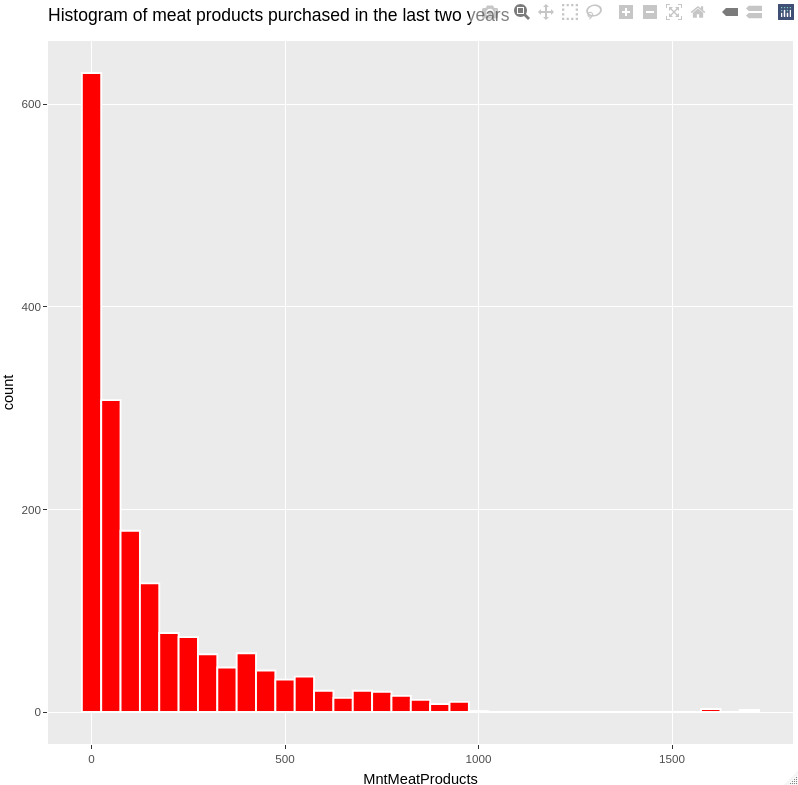
\includegraphics[width=0.7\textwidth]{Img/eda/EDA020.png}
            \end{subfigure}\\
            \begin{subfigure}{\textwidth}
            \centering
            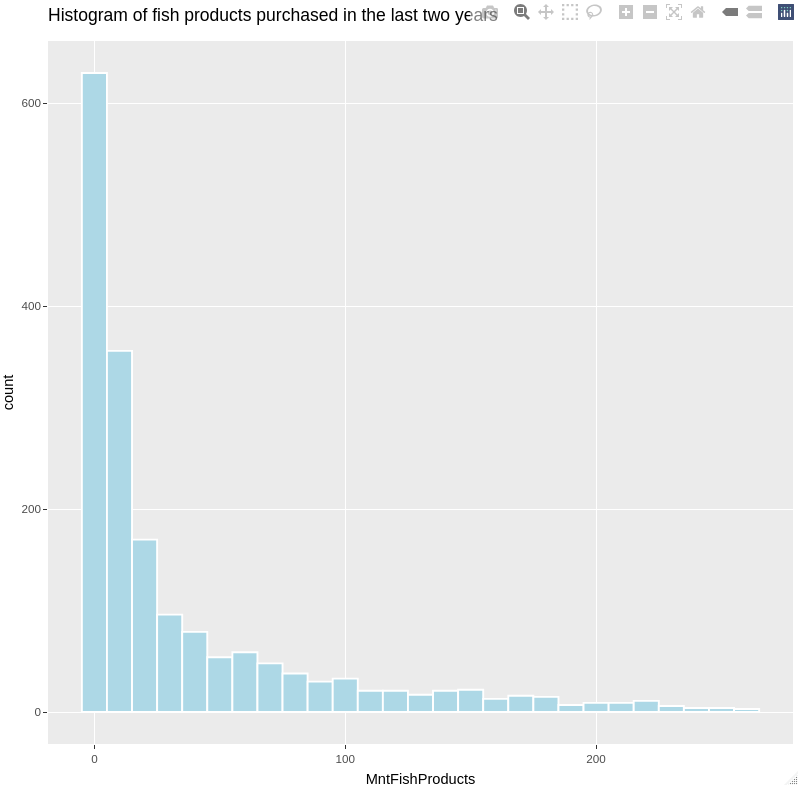
\includegraphics[width=0.7\textwidth]{Img/eda/EDA021.png}
            \end{subfigure}%   
        \end{minipage}
        \hfill
        \begin{minipage}{.3\textwidth}
            \begin{subfigure}{\textwidth}
            \centering
            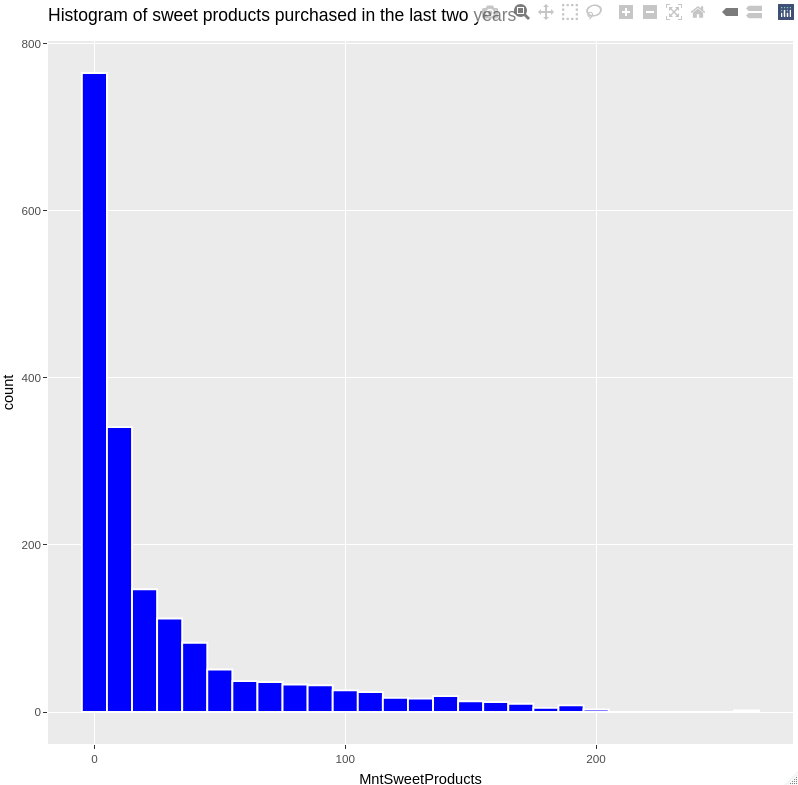
\includegraphics[width=0.7\textwidth]{Img/eda/EDA022.png}
            \end{subfigure}\\
            \begin{subfigure}{\textwidth}
            \centering
            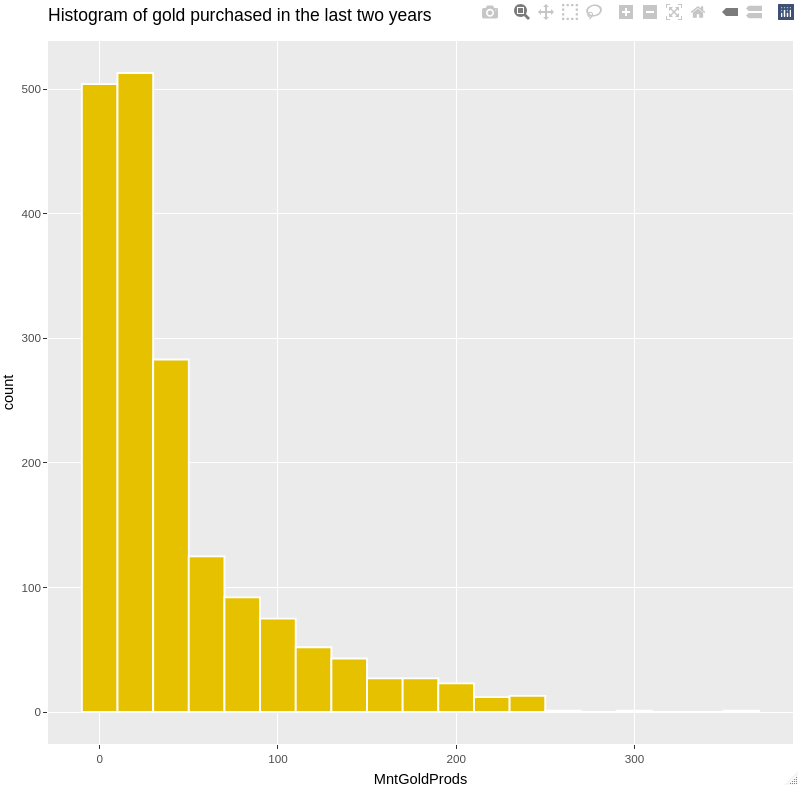
\includegraphics[width=0.7\textwidth]{Img/eda/EDA023.png}
            \end{subfigure}
        \end{minipage}%
    \end{figure}
\end{frame}
%---------------------------------------------------------------------------%
\begin{frame}[fragile]
\frametitle{EDA: Age, Education  e Marital\_Status}
\begin{figure}[!htb]
\minipage{0.32\textwidth}
  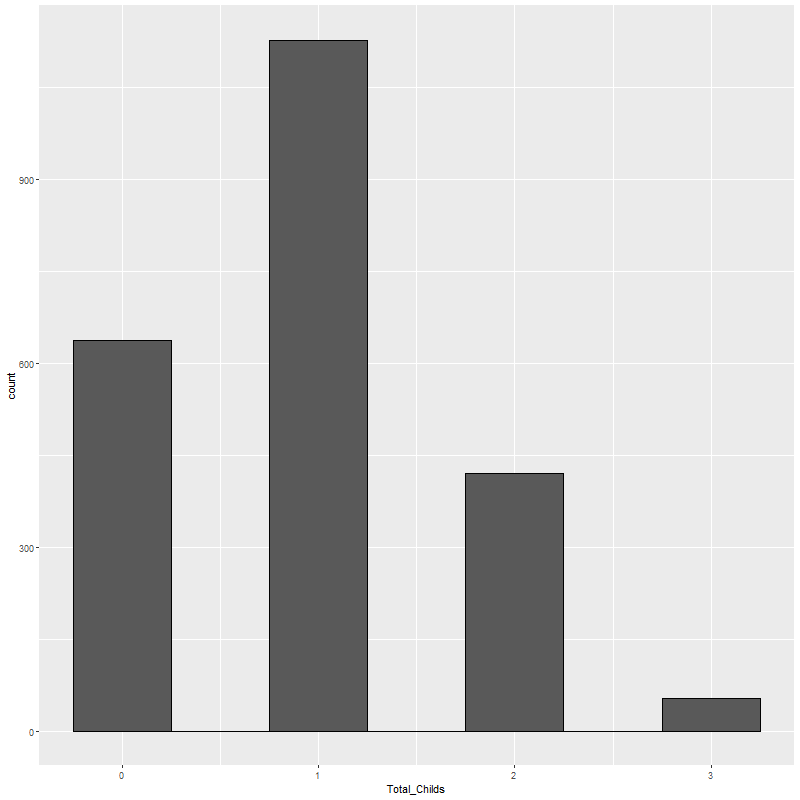
\includegraphics[width=\linewidth]{Img/eda/EDA009.png}
  \caption{Grafico a barre di \textit{Total\_Childs}}\label{fig:BarPlotTc}
\endminipage\hfill
\minipage{0.32\textwidth}
  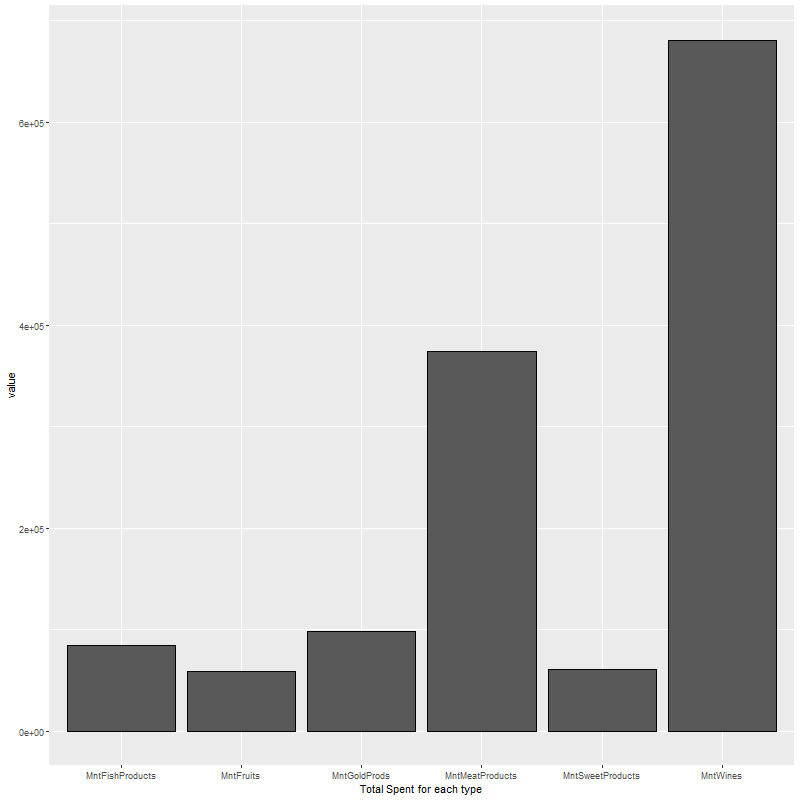
\includegraphics[width=\linewidth]{Img/eda/EDA017.png}
  \caption{Grafico a barre del totale speso per ogni tipo di prodotto}\label{fig:BarPlotTs}
\endminipage\hfill
\minipage{0.32\textwidth}%
  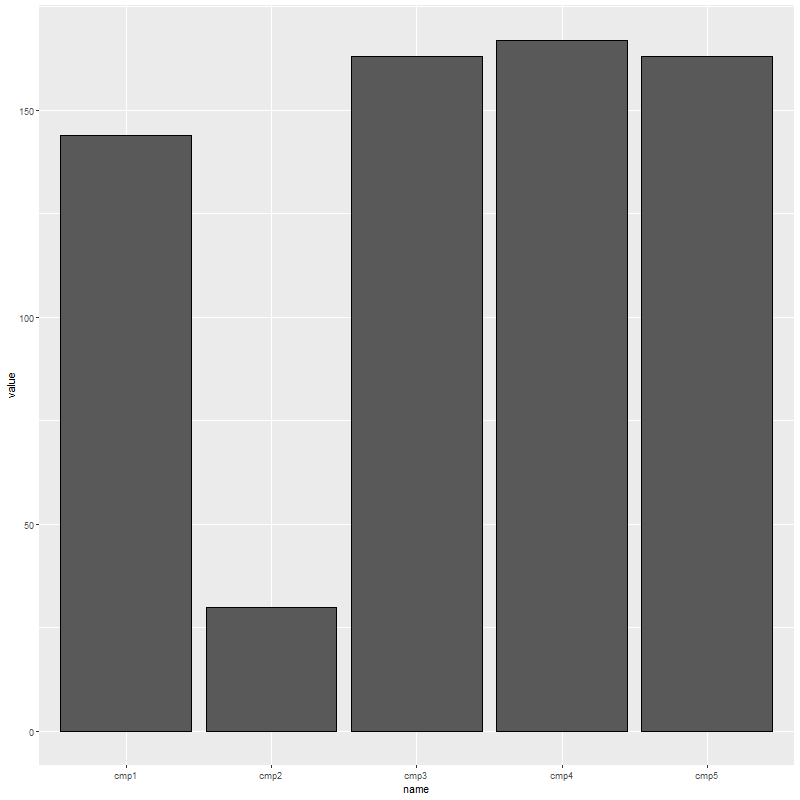
\includegraphics[width=\linewidth]{Img/eda/EDA045.png}
  \caption{Grafico a barre del totale di istanze che hanno accettato la campagna i-esima}\label{fig:BarPlotMt}
\endminipage
\end{figure}

\end{frame}
%---------------------------------------------------------------------------%
\begin{frame}[fragile]
\frametitle{PCA: Varianza spiegata da ogni dimensione}
\begin{minipage}{0.45\textwidth}
\begin{figure}[H]
    \centering
    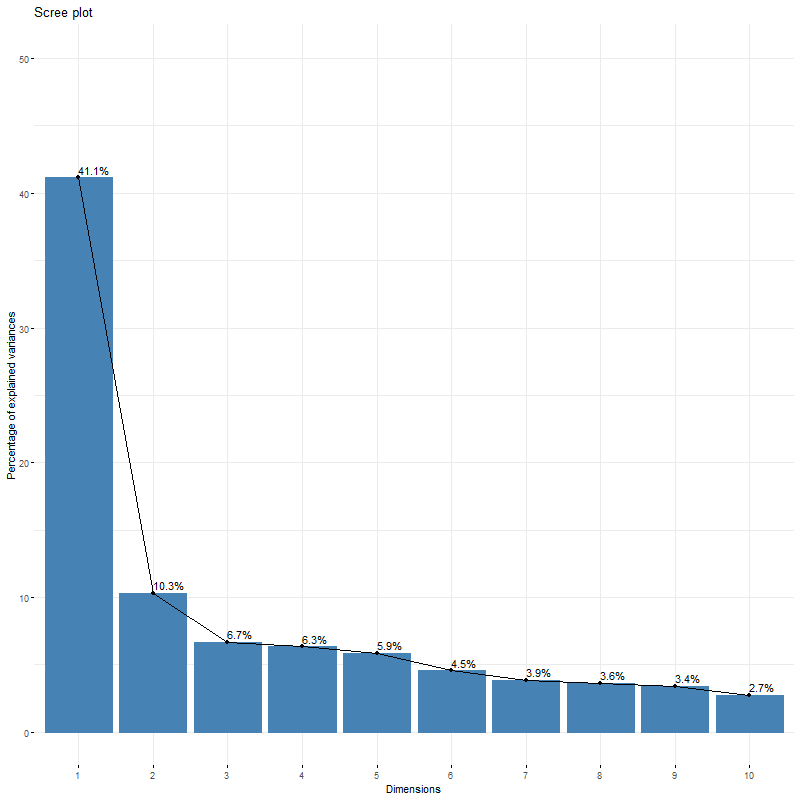
\includegraphics[width=0.8\textwidth]{Img/PCA001.png}
    \caption{Varianza spiegata da ogni Dimensione}
\end{figure}
\end{minipage}%
\hspace{2em}
\begin{minipage}{0.45\textwidth}
\begin{table}[H]
\centering
\begin{tabular}{rrrr}
  \hline
 & eig. & v.p. & c.v.p. \\ 
  \hline
Dim.1 & 7.00 & 41.15 & 41.15 \\ 
  Dim.2 & 1.75 & 10.31 & 51.46 \\ 
  Dim.3 & 1.14 & 6.69 & 58.15 \\ 
  Dim.4 & 1.08 & 6.34 & 64.49 \\ 
  Dim.5 & 1.00 & 5.86 & 70.34 \\ 
  ... & ... & ... & ... \\
   \hline
\end{tabular}
\caption{Output funzione \textit{get\_eigenvalue(pca)}}
\label{fig:get_eigenvalue(pca)}
\end{table}
\end{minipage}%
\end{frame}

%---------------------------------------------------------------------------%
\begin{frame}[fragile]
\frametitle{PCA: Varianza spiegata per la Dim1}
\begin{minipage}{0.45\textwidth}
\begin{figure}[H]
    \centering
    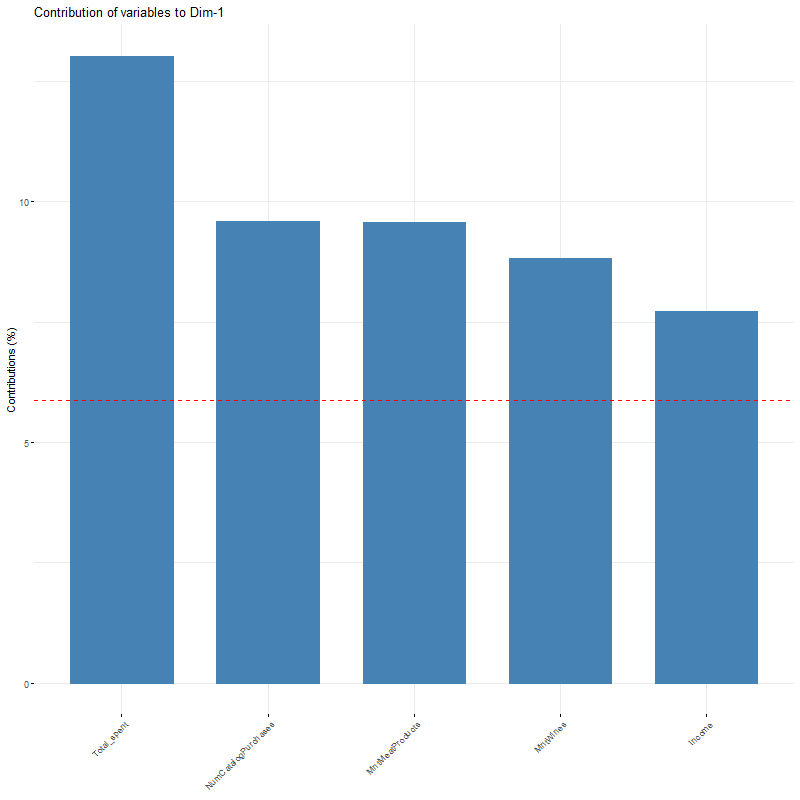
\includegraphics[width=0.7\textwidth]{Img/PCA002.png}
    \caption{Varianza spiegata dalle variabili per la prima dimensione}
    \label{fig:fviz_contrib(pca, choice = "var", axes = 1, top = 5)}
\end{figure}
\end{minipage}%
\hspace{3em}
\begin{minipage}{0.45\textwidth}
\begin{enumerate}
    \item Total\_Spent
    \item MntMeatProducts
    \item NumCatalogPurchases
    \item MntWines 
    \item Income
\end{enumerate}
\end{minipage}%
\end{frame}

%---------------------------------------------------------------------------%
% \begin{frame}[fragile]
% \frametitle{Creazione di nuove variabili riassuntive}
% \begin{table}[H]
% \centering
% \begin{tabular}{rrrr}
%   \hline
%  & Total\_spent & Total\_Campains & Total\_Childs \\ 
%   \hline
% 1 & 1617 &   0 &   0 \\ 
%   2 &  27 &   0 &   2 \\ 
%   3 & 776 &   0 &   0 \\ 
%   4 &  53 &   0 &   1 \\ 
%   5 & 422 &   0 &   1 \\ 
%   6 & 716 &   0 &   1 \\ 
%   \hline
% \end{tabular}
% \caption{Primi valori delle variabili Total\_spent \& Total\_Campains \& Total\_Childs}
% \label{fig:Totalspent&TotalCampains&TotalChilds}
% \end{table}

% \end{frame}


%---------------------------------------------------------------------------%
% \begin{frame}[fragile]
% \frametitle{Refactor: Eliminazione di dati ridondanti}
% \begin{minipage}{0.45\textwidth}
% \begin{table}[H]
% \centering
% \begin{tabular}{rl}
%   \hline
%  & unique(dataSet\$Marital\_Status) \\ 
%   \hline
% 1 & Single \\ 
%   2 & Together \\ 
%   3 & Married \\ 
%   4 & Divorced \\ 
%   5 & Widow \\ 
%   6 & Alone \\ 
%   7 & Absurd \\ 
%   8 & YOLO \\ 
%   \hline
% \end{tabular}
% \caption{Output $unique(dataSet\$Marital\_Status)$}
% \label{fig:unique(dataSetMaritalStatus)}
% \end{table}
% \end{minipage}%
% \hspace{2em}
% \begin{minipage}{0.45\textwidth}
% \begin{table}[H]
% \centering
% \begin{tabular}{rl}
%   \hline
%  & unique(dataSet\$Education) \\ 
%   \hline
% 1 & Graduation \\ 
%   2 & PhD \\ 
%   3 & Master \\ 
%   4 & Basic \\ 
%   5 & 2n Cycle \\ 
%   \hline
% \end{tabular}
% \caption{Output $unique(dataSet\$Education)$}
% \label{fig:unique(dataSetEducation)}
% \end{table}
% \end{minipage}%
% \end{frame}
% %---------------------------------------------------------------------------%
% \begin{frame}[fragile]
% \frametitle{Refactor: Eliminazione di dati ridondanti}
% \begin{minipage}{0.45\textwidth}
% \begin{table}[H]
% \centering
% \begin{tabular}{rl}
%   \hline
%  & unique(dataSet\$Education) \\ 
%   \hline
% 1 & graduate \\ 
%   2 & non-graduate \\ 
%   \hline
% \end{tabular}
% \caption{Output $unique(dataSet\$Education)$ dopo la procedura di \textit{collapsing} dei dati}
% \label{fig:unique(dataSetEducation)2}
% \end{table}
% \end{minipage}%
% \hspace{2em}
% \begin{minipage}{0.45\textwidth}
% \begin{table}[H]
% \centering
% \begin{tabular}{rl}
%   \hline
%  & unique(dataSet\$Marital\_Status) \\ 
%   \hline
% 1 & Single \\ 
%   2 & Couple \\ 
%   \hline
% \end{tabular}
% \caption{Output $unique(dataSet\$Marital\_Status)$ dopo la procedura di \textit{collapsing} dei dati}
% \label{fig:unique(dataSetMaritalStatus)2}
% \end{table}
% \end{minipage}%
% \end{frame}